
\chapter{系统设计}
\label{chap:sys-design}

\section{设计目标}
\label{sec:design-goal}
提出一个实用的生物特征图像安全检索系统用到的检索与加解密算法,并由可靠
的部件与模块实现它,在实现典型的基于内容的图像检索系统的基础上,确保系
统内图像的内容安全性,其检索性能不受加密处理影响。

系统的安全性即,一般权限人可以对图像检索系统进行数据上的管理,如取出系
统中的密图、或密图的特征向量并利用密图的特征向量进行图像匹配等,但一般
权限人无法理解图像内容,只有图像所有人利用加密密钥计算出解密序列对图像
解密后才能获得可以理解的图像。

具体地,本系统分为两部分,即客户端和服务端。

在实现上述目标的同时,客户端应有用户友好的但尽量简洁的、稳定的、健壮的
图形用户界面,以保证客户端程序的可用性。

服务端应有高速可靠的服务器程序做底层以便即使对客户端程序的请求做及时的
响应。

同时客户端与服务端之间应该有可靠的交流协议,以更好的利用网络资源。

\section{系统说明}
\label{sec:sys-description}
% Data flow diagram
% Author: David Fokkema
\pgfdeclarelayer{background}
\pgfdeclarelayer{foreground}
\pgfsetlayers{background,main,foreground}

\begin{figure}[H]

\centering
\begin{tikzpicture}[
font=\sffamily,
    every matrix/.style={ampersand replacement=\&,column sep=1cm,row sep=1cm},
    source/.style={draw,thick,rounded corners,fill=red!20,inner sep=.3cm},
    process/.style={draw,thick,rounded corners,inner sep=.3cm,fill=blue!20},
    sink/.style={source,fill=green!20},
    to/.style={->,>=stealth',shorten >=1pt,semithick,font=\sffamily\footnotesize},
    every node/.style={align=center}]

    % Position the nodes using a matrix layout
    \matrix{
        \& \& \node[source] (inputimg) {录入图像}; \& \\
        \& \& \node[process] (correction) {矫正}; \& \\
        \node[source] (restoredimg) {还原图};
        \& \node (hiddennodeclient) {};
        \& \node[source] (ainputimg) {待添加图像};
        \& \node[source] (rinputimg) {待检索图像}; \\
          \node[process] (decimg) {解密 (逆置乱)};
        \& \& \node[process] (encimg) {加密 (置乱)};
        \& \node[process] (encimga) {加密 (置乱)}; \\
    \node (hiddenhttpa) {}; \& \node (hiddenhttpb) {};
      \& \node (hiddenhttpc) {}; \& \node (hiddenhttpd) {}; \\
    \node (hiddennodeserver) {};
       \& \& \node[process] (extfeat) {提取特征}; 
       \& \node[process] (extfeata) {提取特征}; \\
    \node[source] (results) {匹配结果};
        \& \node[sink] (imgdb) {图片数据库};
        \& \node[sink] (featdb) {特征数据库};
        \& \node (rightbottom) {}; \\
  };

  \path (hiddennodeclient.south) + (0, -0.5) node (client)
      {\Large \emph{客户端}};
  \path (hiddennodeserver.east) + (1.8, -0.2) node (server) {\Large
     \emph{服务端}};
  \path (hiddenhttpa.east) + (1.8, 0) node (http-level)
      {\Large \emph{HTTP}};

  % Draw the arrows between the nodes and label them.
  \draw[to] (decimg) -- (restoredimg);
  \draw[to] (results) -- (decimg);
  \draw[to] (inputimg) -- (correction);
  \draw[to] (correction) -- (ainputimg);
  \draw[to] (ainputimg) -- (encimg);
  \draw[to] (encimg) -| node[midway, above] {加入} (imgdb);
  \draw[to] (encimg) -- (extfeat);
  \draw[to] (extfeat) -- node[midway, left] {加入} (featdb);
  \draw[to] (rinputimg) -- (encimga);
  \draw[to] (encimga) -- (extfeata);
  \draw[to] (extfeata) |- node[midway, below] {比对} (featdb);
  \draw[to] (featdb) -- (imgdb);
  \draw[to] (imgdb) -- (results);

  \begin{pgfonlayer}{background}
    \path (decimg.west |- rinputimg.north) + (-0.3, 0.3) node
    (a) {};
    \path (encimg.south -| rinputimg.east) + (+0.3, -0.3) node (b)
    {};
    \path[fill=cyan!10, rounded corners, draw=black!50, dashed] (a)
    rectangle (b);
    \path (extfeat.north -| extfeata.east) + (+0.5, +0.3) node (a) {};
    \path (results.west |- imgdb.south) + (-0.7, -0.3) node (b) {};
    \path[fill=yellow!10, rounded corners, draw=black!50, dashed] (a)
    rectangle (b);
    \path (hiddenhttpa.west |- hiddenhttpd.north) + (-1.7, 0.3) node
    (a) {};
    \path (hiddenhttpc.south -| hiddenhttpd.east) + (+1.5, -0.3) node
    (b) {};
    \path[fill=gray!10, rounded corners, draw=black!50, dashed] (a)
    rectangle (b);
  \end{pgfonlayer}

\end{tikzpicture}

\caption{系统流程图示}
\label{fig:sys-workflow}
\end{figure}


如图所示,系统由客户端和服务端构成。

其中客户端所实现的功能有:
\begin{itemize}
\item 加密(置乱图像)
\item 解密(逆置乱图像)
\end{itemize}

服务端所实现的功能有:
\begin{itemize}
\item 提取输入图像的特征
\item 将密图加入图片数据库
\item 将特征加入特征数据库
\item 比对特征数据库中的特征
\end{itemize}

客户端与服务端通过HTTP协议进行交互,必要时可以使用HTTPS协议来增加安全
性而无需修改大量代码。其中,客户端与服务端之间也有构建于HTTP之上的应用
协议。流程如下:
% Data flow diagram
% Author: David Fokkema
\pgfdeclarelayer{background}
\pgfdeclarelayer{foreground}
\pgfsetlayers{background,main,foreground}

\begin{figure}[H]
\centering
\begin{tikzpicture}[
font=\sffamily,
    every matrix/.style={ampersand replacement=\&,column sep=1cm,row sep=1cm},
    source/.style={draw,thick,rounded corners,fill=red!20,inner sep=.3cm},
    process/.style={draw,thick,rounded corners,inner sep=.3cm,fill=blue!20},
    entity/.style={source,fill=green!20},
    post/.style={source,fill=gray!20},
    to/.style={->,>=stealth',shorten >=1pt,semithick,font=\sffamily\footnotesize},
    every node/.style={align=center}]

  % Position the nodes using a matrix layout
  \matrix{
        \node[source] (ret-img) {待检索图片};
     \& \node[entity] (client) {客户端};
     \& \node[source] (upload-img) {待上传图片};
     \& \node[source] (restored-img) {还原图}; \\
        \& \node[process] (enc-img) {加密图片};
     \& \& \node[process] (dec-img) {解密图片}; \\
        \& \node[process] (base64-enc) {base64编码};
     \& \& \node[process] (base64-dec) {base64解码}; \\
        \node[post] (add) {/add};
     \& \node[post] (send) {/send};
     \& \node[post] (retrieve) {/retrieve}; \\
        \node[process] (add-to-db) {加入数据库};
     \& \node[process] (prepare) {准备结果集};
     \& \node[entity] (res-set) {结果集};
     \& \node (hidden-row-5) {}; \\
  };

  % Draw the arrows between the nodes and label them.
  \draw[to] (upload-img) -- (client);
  \draw[to] (ret-img) -- (client);
  \draw[to] (client) -- (enc-img);
  \draw[to] (enc-img) -- (base64-enc);
  \draw[to] (base64-enc) -- (send);
  \draw[to] (base64-enc) -| (add);
  \draw[to] (send) -- (prepare);
  \draw[to] (add) -- (add-to-db);
  \draw[to] (retrieve) -- (res-set);
  \draw[to] (res-set) -| (base64-dec);
  \draw[to] (base64-dec) -- (dec-img);
  \draw[to] (dec-img) -- (restored-img);
  \draw[to] (prepare) -- (res-set);
\end{tikzpicture}

\caption{系统流程图示}
\label{fig:app-workflow}
\end{figure}



具体地,本系统的协议详细如下表。

\begin{center}
    \begin{longtable}{| l | p{2.5cm} | p{2.5cm} | p{5cm} |}
    \hline
    \textbf{URL} & \textbf{参数} & \textbf{返回} & \textbf{说明} \\
    \hline
    \endfirsthead
    \multicolumn{4}{r}{\textit{接上页}} \\
    \hline
    \textbf{URL} & \textbf{参数} & \textbf{返回} & \textbf{说明} \\
    \hline
    \endhead
    \hline
    \endfoot
    \endlastfoot
    \texttt{/login}
  & 由客户端生成的id
  & status
  & 必须在客户端初始化后立即调用,使得服务端可以登记客户端id \\
    \hline
    \texttt{/logout}
  & 无
  & status
  & 必须在客户端关闭前调用,使得服务端可以根据post的cookies注销客户端id \\
    \hline
    \texttt{/add}
  & base64编码后的图像
  & status
  & 添加新图片至服务端时使用 \\
    \hline
    \texttt{/send}
  & base64编码后的图像
  & 结果个数
  & 将待检索图像送至服务端,接到此请求后,
    服务端根据匹配算法立刻开始准备结果集,并等待
    客户端发送\texttt{/retrieve}请求 \\
    \hline
    \texttt{/retrieve}
  & 无
  & base64编码后的图像与图像与原图距离
  & 在客户端发送\texttt{/send}请求并收到回复后,即可发送该请求来获取结果
    图像 \\
    \hline
  \caption{应用协议定义} \\
  \end{longtable}
  \label{tab:app-proto-def}
\end{center}




\section{功能原理}
\label{sec:func-impl}

为了标准化图片库,便于实现功能,本系统只接受宽$640$像素,高
$480$像素,即$4:3$的灰度JPEG图片。

\subsection{检索匹配方面}
\label{sec:retrieval-impl}
本系统利用二维DCT抽取出一张图片的特征向量。具体方法如下:
\begin{enumerate}
\item 将输入JPEG图片按$8 \times 8$分块,对每块做DCT;
\item 取每块的DC系数,添加到数组$V$中;
\item 将$V$按降序排序,得到$W$,并取$W$的前$n$个元素作为该输入图片的特
  征向量。
\end{enumerate}

其中$n$可以根据实际需要来取。由于$W$中下标越大的元素,其值越小,在向量
距离计算中起到的作用就越小,因此本系统实现中对检索效果和效率进行衡量,
选择了$128$作为该参数的值。

计算距离方面使用的是numpy库中的\texttt{linalg.norm}函数。

\subsection{加解密方面}
\label{sec:enc-dec-impl}
本系统使用的加解密算法的初始密钥由三组$x_0$,$r$,$s$组成,
其中$x_0 \in (-1, 1)$,$r \in [3.57, 4]$,$s > 0, s \in \mathbb{Z}$。

加密算法首先使用伪随机序列生成算法生成若干置乱表,然后根据置乱表对图片
进行块内和块间的置乱达到使图片不可理解、但保留DC系数的统计特性的目的。
解密算法与加密算法类似,只是使用的置乱表不一样,即加解密算法是对合的。

由Logistic映射生成具有$n$个元素的伪随机序列的具体做法\cite{lu2007}是:
\begin{enumerate}
  \item 使用初始密钥$x_0$和$r$,迭代Logistic公式,生成具有$n + s$个元
      素的混沌序列,并舍去前$s$个元素,得到$L = \{x_1, x_2, x_3, \dotsc, x_n\}$;
  \item 对$L$进行升序排序,得到$M = \{x_1^\prime, x_2^\prime, x_3^\prime,
      \dotsc, x_n^\prime\}$;
  \item 定位$x_i$在$x_i^\prime$中的位置序数,得到序数序列,记为$P =
      \{p_1, p_2, p_3, \dotsc, p_n\}$
\end{enumerate}
$P$就是所求的关于初始密钥$x_0$、$r$和$s$的伪随机序列。

由置乱表生成逆置乱表的具体做法是:
\begin{enumerate}
  \item 扩展输入序列为$P^\prime = \{(0, x_1), (1, x_2), (2, x_3),
      \dotsc, (n - 1, x_n)\} \quad x_i \in P$;
  \item 建立一个新表$I$,使得$\forall (i, x_{i + 1}) \in P^\prime$,
      $I_{x_{i + 1}} = i$
\end{enumerate}
$I$就是所求的关于$P$的逆置乱表。

本系统为了保证每个DCT块的均值不变,利用不同的初始密钥生成了3个伪随机序列,分别是:
\begin{itemize}
  \item 利用第一组初始密钥生成了具有64个元素的$T_{block}$,作为DCT块内的
    置乱表;
  \item 利用第二组初始密钥生成了具有$h$个元素的$T_{row}$,作为块间的行
    置乱表;
  \item 利用第三组初始密钥生成了具有$w$个元素的$T_{column}$,作为块间
    的列置乱表;
\end{itemize}
其中$w$等于图片宽度除以$8$,$h$等于图片宽度除以$8$。

\section{系统架构与实现}
\label{sec:sys-arch}
\subsection{客户端}
客户端架构如下图

\begin{figure}[H]
\centering
\begin{tikzpicture}[
  level distance=130pt,
  font=\sffamily,
  basic/.style={draw,text width=2cm,drop shadow,font=\sffamily,rectangle},
  root/.style={basic,rounded corners=2pt,thin,align=center,fill=green!30},
  level 2/.style={basic,rounded
    corners=6pt,thin,align=center,fill=green!50,sibling distance=5mm,
    text width=6em},
  level 3/.style={basic,thin,align=left,fill=cyan!20,text width=10em},
  level 1/.style={sibling distance=10mm,level distance=100pt, text width=5em},
  edge from parent/.style={->,draw},
  grow'=right,
  >=latex]

\Tree [.\node[root] {客户端};
          [.\node[level 2] {前端};
              [.\node[level 3] (ui-node) {\texttt{ui.py}}; ]
              [.\node[level 3] (ui-comp-node)
              {\texttt{libs/ui\_comp.py}}; ] ]
          [.\node[level 2] {核心};
              [.\node[level 3] (core-node) {\texttt{libs/core.py}}; ]
              [.\node[level 3] (logistic-node) {\texttt{libs/logistic.py}}; ] ] ]
\end{tikzpicture}
\caption{客户端架构图示}
\label{fig:client-arch}
\end{figure}



\texttt{ui.py}内有类\texttt{SecureRetrievalUI},是客户端的主界面类。

\texttt{libs/ui\_comp.py}内含有多个类,是客户端前端的辅助模块,用于图像的
显示等,如下表

\begin{table}[H]
  \centering
  \begin{tabular}{| l | p {7cm} |}
    \hline
    类名 & 说明 \\ \hline
    \texttt{ResultListItemDelegate} & 用于结果列表的显示委托类 \\ \hline
    \texttt{Counter} & 用于多线程中返回的结果数的计数类 \\ \hline
    \texttt{ResultListModel} & 用于为结果列表提供数据源模型 \\ \hline
    \texttt{ImageWidget} & 用于在用户界面中显示图像 \\ \hline
    \texttt{LoggerHandler} & 用于将\texttt{Logger}的日志信息重定向至用户界面中的
    日志对话框 \\ \hline
    \texttt{ColoredFormatter} & 用于格式化\texttt{Logger}的日志信息 \\ \hline
  \end{tabular}
%  \caption{\texttt{libs/ui\_comp.py}文件主要内容}
  \label{tab:client-ui-comp}
\end{table}



\texttt{libs/core.py}内有类\texttt{ClientCore},是客户端的功能核心。该
类主要方法有
\begin{table}[H]
  \centering
  \begin{tabular}[H]{| l | p{3.5cm} | p{3cm} | p{4cm} |}
    \hline
    方法名 & 参数 & 返回 & 说明 \\
    \hline
    \texttt{open\_img} & \texttt{path:} 图像路径
  & \texttt{np.ndarray}型的灰度矩阵表示打开的图像 & 用于打开给定路径的JPEG文件 \\
    \hline
    \texttt{save\_img} & \texttt{path:} 保存路径\newline
    \texttt{img:} 灰度矩阵 & 无 & 用于按JPEG格式保存给定的灰度矩阵 \\
    \hline
    \texttt{\_transform} & \texttt{img:} 灰度矩阵\newline
                           \texttt{table:} 块间置乱表\newline
                           \texttt{block\_table:} 块内置乱表\newline
  & \texttt{np.ndarray}型的按照给定的表置乱后的矩阵 & 主置乱函数,\newline
    \texttt{enc\_img}与\texttt{dec\_img}\newline
    都是在这个方法的基础上实现的 \\
    \hline
    \texttt{upload\_img} & \texttt{raw:} 待上传图像的二进制数据
  & 服务器返回的json & 用于上传图像 \\
    \hline
    \texttt{send\_img} & \texttt{raw:} 待检索的二进制数据\newline
                         \texttt{max\_count:} 最大结果数,默认为10
  & 服务器返回的json & 用于检索图像 \\
    \hline
    \texttt{parse\_result} & 无 & 服务器返回图像的二进制数据与该图像与
    原图的距离 & 用于获取服务器准备好的结果,每次调用获取一个 \\
    \hline
  \end{tabular}
%  \caption{\texttt{ClientCore}主要方法}
  \label{tab:client-core}
\end{table}



\texttt{LogisticPermutation}类用于根据给定的初始密钥生成加解密置换表。
\texttt{ClientCore}依赖于\texttt{LogisticPermutation}类
(\texttt{libs/logistic.py})为其生成加解密置换表以便加解密使用。
根据初始密组生成加解密置换表的方法见\ref{sec:enc-dec-impl}。

\subsection{服务端}
服务端架构如下图

\begin{figure}[H]
\centering
\begin{tikzpicture}[
font=\sffamily,
  basic/.style={draw,text width=2cm,drop shadow,font=\sffamily,rectangle},
  root/.style={basic,rounded
    corners=2pt,thin,align=center,fill=green!30},
  level 2/.style={basic,rounded
    corners=6pt,thin,align=center,fill=green!50, text width=6em},
  level 3/.style={basic,thin,align=left,fill=cyan!20,align=center,
    text width=10em},
  level 1/.style={sibling distance=10mm,text width=5em},
  edge from parent/.style={->,draw},
  >=latex]

\Tree [.\node[root] {服务端};
          [.\node[level 2] {http服务器};
              [.\node[level 3] {\texttt{server.py}}; ] ]
          [.\node[level 2] {核心};
              [.\node[level 3] {\texttt{core.py}}; ] ] ]

\end{tikzpicture}
\caption{服务端架构图示}
\label{fig:server-arch}
\end{figure}



源文件\texttt{server.py}在代码层面上定义了应用协议的具体行为。各URL含
义参见\ref{tab:app-proto-def}。

\texttt{core.py}内容见下表

\begin{table}[H]
  \centering
  \begin{tabular}{| l | p {7cm} |}
    \hline
    \textbf{类名} & \textbf{说明} \\ \hline
    \texttt{JPEGFileEntry} & 用于SQLAlchemy的ORM类 \\ \hline
    \texttt{ServerCore} & 服务端的功能核心 \\ \hline
  \end{tabular}
  \caption{\texttt{core.py}文件主要内容}
  \label{tab:server-core-py}
\end{table}



数据库引擎选用的是Python自带的SQLite3数据库引擎,无需配置,即装即用,
可以与本系统良好结合。本系统建表一张,表名为\texttt{entries},存储了本
系统所需的每张JPEG图片的信息,具体内容如下表

\begin{table}[H]
  \centering
  \begin{tabular}{| l | l | p {5cm} |}
    \hline
    \textbf{列名} & \textbf{类型} & \textbf{说明} \\ \hline
    \texttt{\_id} & \texttt{Integer} & 主键,自增 \\ \hline
    \texttt{feature\_vector} & \texttt{LargeBinary} & 图片特征向量的二
    进制数据,缓存这个是为了有效提高检索效率 \\ \hline
    \texttt{uuid} & \texttt{String} & 随机生成的UUID,用作图片的实际文
    件名 \\ \hline
    \texttt{fingerprint} & \texttt{String} & Unique,图片的SHA-1指纹,
    用作排重 \\ \hline
  \end{tabular}
  \caption{表\texttt{entries}定义}
  \label{tab:db-entries-def}
\end{table}



\texttt{ServerCore}是服务端的主要功能模块,其主要方法见下表
\begin{table}[H]
  \centering
  \begin{tabular}[H]{| l | p{3.5cm} | p{3cm} | p{3cm} |}
    \hline
    \textbf{方法名} & \textbf{参数} & \textbf{返回} & \textbf{说明} \\
    \hline
    \texttt{\_extract\_feat\_vec}
  & \texttt{img:} 灰度矩阵在按块DCT后的矩阵\newline
    \texttt{n:} 所取的DC系数个数
  & \texttt{np.ndarray}型的特征向量,DC系数按降序排列
  & 用于抽取出给定图像的特征向量 \\
    \hline
    \texttt{prepare\_results}
  & \texttt{data:} base64编码的密图\newline
    \texttt{n:} 结果个数
  & 实际匹配结果个数
  & 用于获取给定图像的匹配结果 \\
    \hline
    \texttt{add\_jpeg\_file}
  & \texttt{data:} base64编码的密图
  & 函数执行状态 & 用于将新图片加入数据库 \\
    \hline
  \end{tabular}
  \caption{\texttt{ServerCore}主要方法}
  \label{tab:server-core}
\end{table}



\section{用户界面简介}
\label{sec:ui-intro}

打开客户端后,会显示如下的图形用户界面
\begin{figure}[H]\centering
  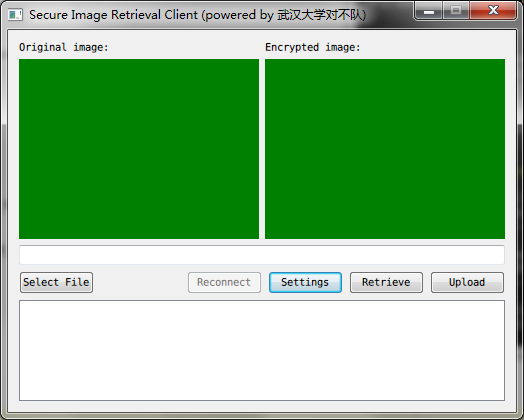
\includegraphics[keepaspectratio=true]{images/ui-connected.png}
  \caption{用户界面}
\label{fig:ui-connected}
\end{figure}

注意:如果未能与服务器连接成功,则\texttt{Retrieve}与\texttt{Upload}按
钮不可用,\texttt{Reconnect}可用,如下图,此时应
点击\texttt{Settings}按钮打开设置面板以检查服务器地址是否正确,确认完毕
后,点击\texttt{Ok}按钮确认,随后点击\texttt{Reconnect}以试图重新连接服
务器。若连接成功,则\texttt{Reconnect}变为不可用状
态,\texttt{Retrieve}与\texttt{Upload}变为可用状态。

\begin{figure}[H]
  \centering
  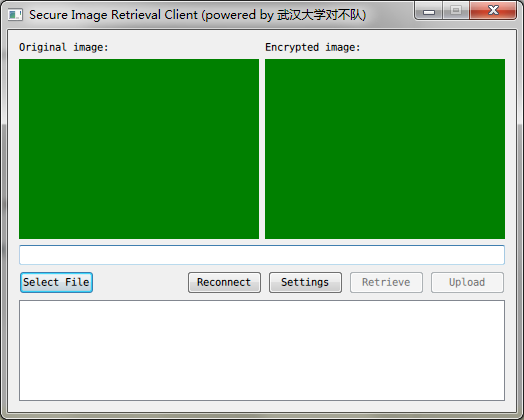
\includegraphics[keepaspectratio=true]{images/ui-disconnected.png}
  \caption{未连接服务器的客户端}
  \label{fig:ui-disconnected}
\end{figure}

配置界面\texttt{Settings}如下图

\begin{figure}[H]
  \centering
  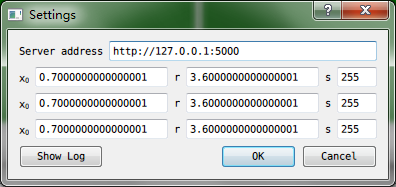
\includegraphics[keepaspectratio=true]{images/ui-settings-dialog.png}
  \caption{配置界面}
  \label{fig:ui-settings-dialog}
\end{figure}

服务器地址(形式为一个URL),与三组密钥均在此设置。密钥设置要求
见\ref{sec:enc-dec-impl}。如果服务器地址被改变,并且客户端已经连接到服
务器,客户端会与原服务器断开连接并试图连接新服务器。配置界面
的\texttt{Show Log}按钮可以打开一个日志窗口,记录了客户端的运行情况。
日志窗口\texttt{Log}如下图

\begin{figure}[H]
  \centering
  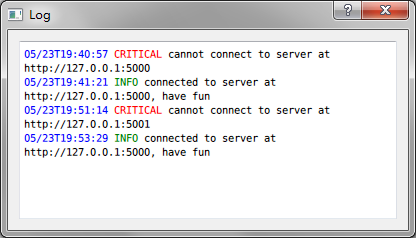
\includegraphics[keepaspectratio=true]{images/ui-log-dialog.png}
  \caption{日志窗口}
  \label{fig:ui-log-dialog}
\end{figure}

当用户通过\texttt{Select File}按钮选择一张图片后,该图片与密图会同时显
示出来,如下图

\begin{figure}[H]
  \centering
  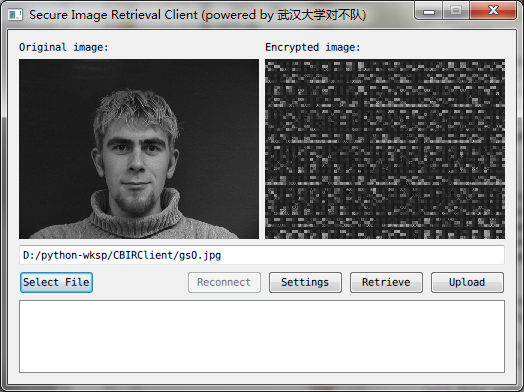
\includegraphics[keepaspectratio=true]{images/ui-image-selected.png}
  \caption{选择一张图片后}
  \label{fig:ui-image-selected}
\end{figure}

此时用户可以点击\texttt{Upload}来将该文件(密图)上传至服务器,或点击
\texttt{Retrieve}来检索该图片。注意,如果该图片已存在于服务端,服务器
将不会接受该图片。

点击\texttt{Retrieve}按钮后,客户端会发送一个检索请求到服务器,并开始
获取结果。此时客户端会显示状态为\texttt{fetching...},如下图

\begin{figure}[H]
  \centering
  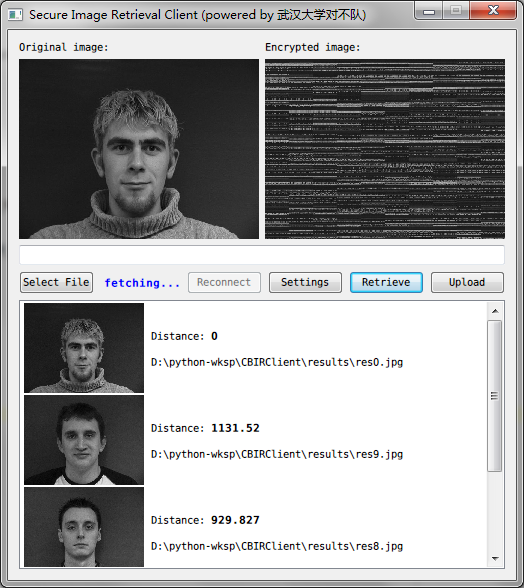
\includegraphics[keepaspectratio=true]{images/ui-retrieve-fetching.png}
  \caption{客户端获取结果中}
  \label{fig:ui-retrieve-fetching}
\end{figure}

当客户端每次获取一个结果,它会将结果解密并保存在工作目录下
的\texttt{results}目录下,文件名为\texttt{res$i$.jpg}。其中$i$不一定是结
果在结果集中的大小序号。当全部结果获取完毕后,客户端会将结果集按升序排序,
并且状态显示为\texttt{done},如下图

\begin{figure}[H]
  \centering
  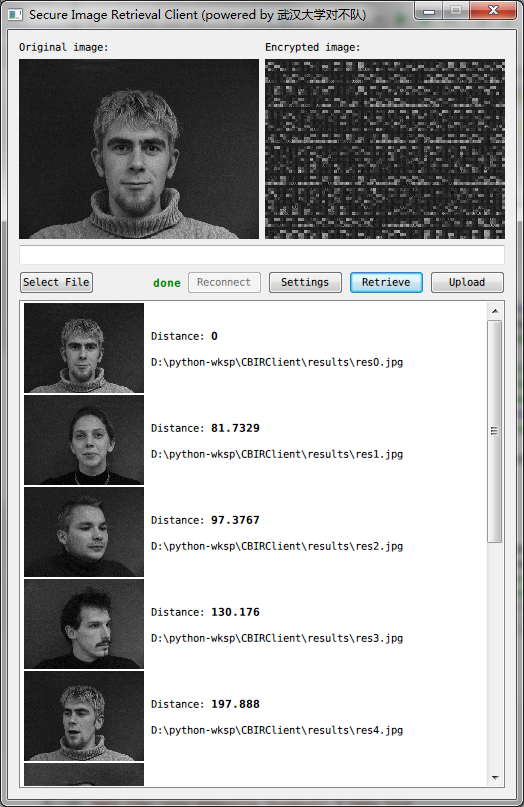
\includegraphics[keepaspectratio=true]{images/ui-retrieve-done.png}
  \caption{客户端获取所有结果后}
  \label{fig:ui-retrieve-done}
\end{figure}

在检索过程中,日志窗口会记录一些有用的信息,如检索耗时与检索结束耗时
(从发送检索请求到所有结果获取结束所耗费的时间)等,如下图


\begin{figure}[H]
  \centering
  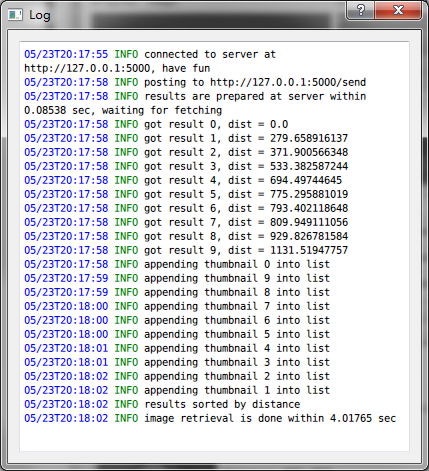
\includegraphics[keepaspectratio=true]{images/ui-retrieve-log.png}
  \caption{检索过程的日志记录}
  \label{fig:ui-retrieve-log}
\end{figure}

